% Extended Data plan: at most 10 items, each cited in the main text. Updated 17 Nov 2026 to match
% paper/decisions.md: eight figures, Extended Data Table 1 (in sections/08-tables.tex) and one free
% slot for the rows still to decide (non-neurological MIMIC-IV, the reasons the agent gives for its
% requests). The thinking test moved to Supplementary Table 11 to keep that slot.

\section*{Extended Data ($\le$10 items; 9 used)}

\role{Hold what a reviewer will ask for but the story does not need; each item backs one claim and is
cited where that claim is made.}

\artefacts
\noindent{\small
\begin{tabularx}{\linewidth}{@{}l>{\raggedright\arraybackslash}Xl>{\raggedright\arraybackslash}p{0.24\linewidth}@{}}
\toprule
Item & Content & Backs & Why \\ \midrule
ED Fig.~1 & The dataset: what a case contains, the 20 conditions and the split, physician review,
  similarity to training & R1 & Dataset quality and leakage \\
ED Fig.~2 & Reward history: the discarded reward versions, what went wrong and what changed & C2 & Shows
  the reward was not tuned until it worked \\
ED Fig.~3 & Inter-physician agreement and a re-checked sample of cases & R1, C3 & The policies are not
  one physician's opinion \\
ED Fig.~4 & Training on other models (Gemma 4 E4B, a smaller Qwen, possibly Granite), one seed & C2 &
  The effect is not specific to one model \\
ED Fig.~5 & Results per condition, with a clinical reading & C2 & No single condition carries the
  effect \\
ED Fig.~6 & Acute against chronic conditions (synthetic cases) & C2 & Where the work-up matters most \\
ED Fig.~7 & Controls: no test, no test menu, scripted agents (perfect, orders everything) & C1, C2 &
  Ends of every scale \\
ED Fig.~8 & Robustness: changed reward weights; cases with contradictory facts & C2 & Not a tuning
  artefact, not surface cues \\
ED Table~1 & Main results on the NeuroBench test and on MIMIC-IV (sections/08-tables.tex) & C2, C4 &
  Every number of Figs.~3 and~5 with CIs and $P$ \\
Free & Non-neurological MIMIC-IV, or the reasons given for each request & -- & Decided from the
  results \\
\bottomrule
\end{tabularx}}

\status{ED Fig.~1 has an October draft (below, to redo in the house style); ED Fig.~2 can be built
now; the others follow the runs and the physician studies.}

\renewcommand{\figurename}{Extended Data Fig.}
\setcounter{figure}{0}

\begin{figure}[p]
\centering
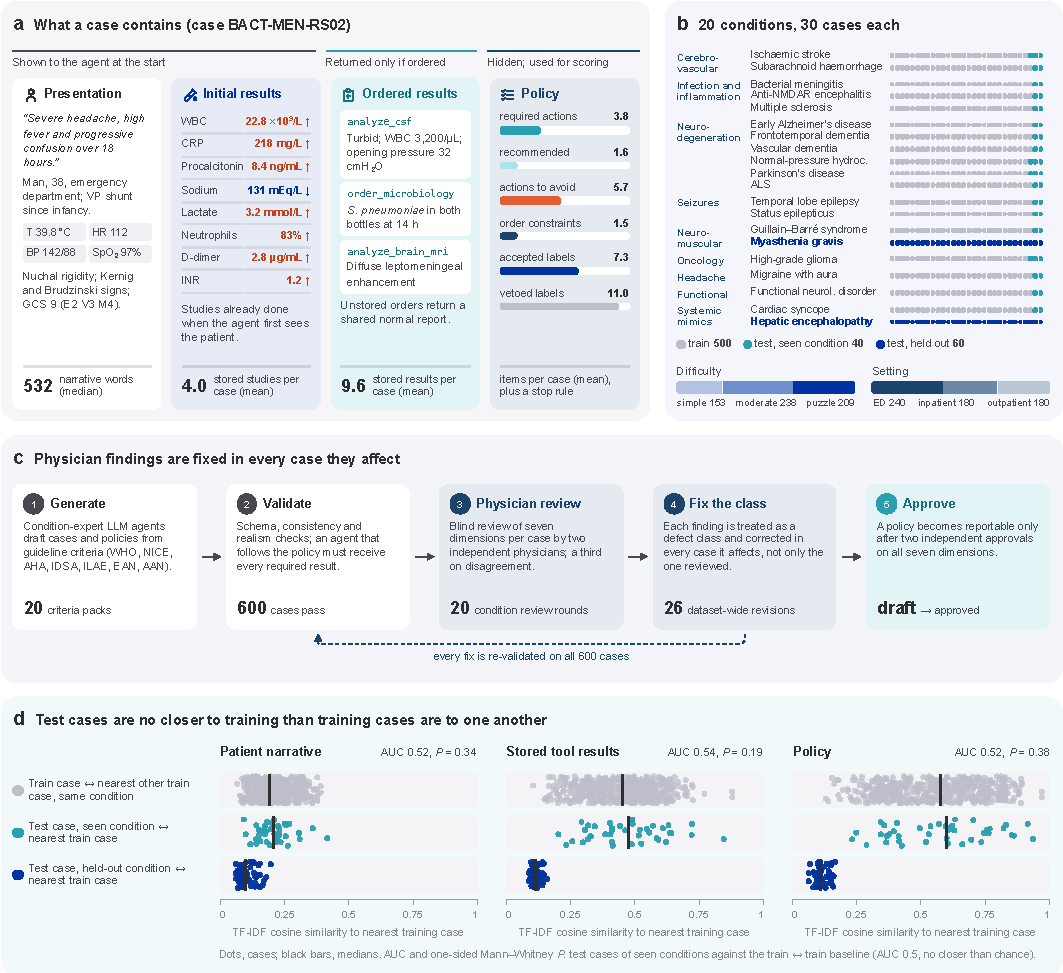
\includegraphics[width=\textwidth]{fig2.pdf}
\caption{\textbf{Draft from October, to redo in the style of Figs.~1--3.} Panels: \textbf{a}, what a
case contains (visible, on order, hidden); \textbf{b}, the 20 conditions and the split; \textbf{c},
generation, validation, blind review, defect-class fixes; \textbf{d}, nearest-neighbour similarity to
training for narrative, results and policy.}
\label{fig:ed-dataset}
\end{figure}
